\section{施工现场事故应急预案}
\subsection{总则}
\subsubsection{编制目的}

为了保障施工生产的正常进行,对潜在的事故作出应急准备与响应。防止施工企业施工现场的生产安全事故发生,完善应急工作机制,在工程项目发生事故状态下,迅速有序地开展事故的应急救援工作,
预防或减少可能造成的人员伤亡或者财产损失,最大限度的控制危险,认真落实“安全第一、预防为主、综合治理”的安全成产方针而制定本预案。

\subsubsection{编制依据}

(1)	《中华人民共和国安全生产法》

(2) 《特种设备事故应急预案编制导则》 GB/T 33942-2017

(3) 《生产经营单位安全生产事故应急预案编制导则》 GB/T 29639-2013

(4) 《生产安全事故应急演练指南》 AQ/T 9007-2011

(5) 建设部 《工程建设重大事故和调查程序规定》

(6) 项目相关规定以及建筑工程安全操作规程

\subsection{应急组织体系}
\subsubsection{事故应急救援组织体系与主要职责}

项目部应急指挥中心领导组下设应急指挥中心办公室,下分七个小组,分别为联络调度组、抢险救援组、医疗救助组、物资保障组、事故调查组与善后组,项目应急指挥组织机构见图 \ref{fig:c8f1}

\begin{figure}[thbp!]
    \centering
    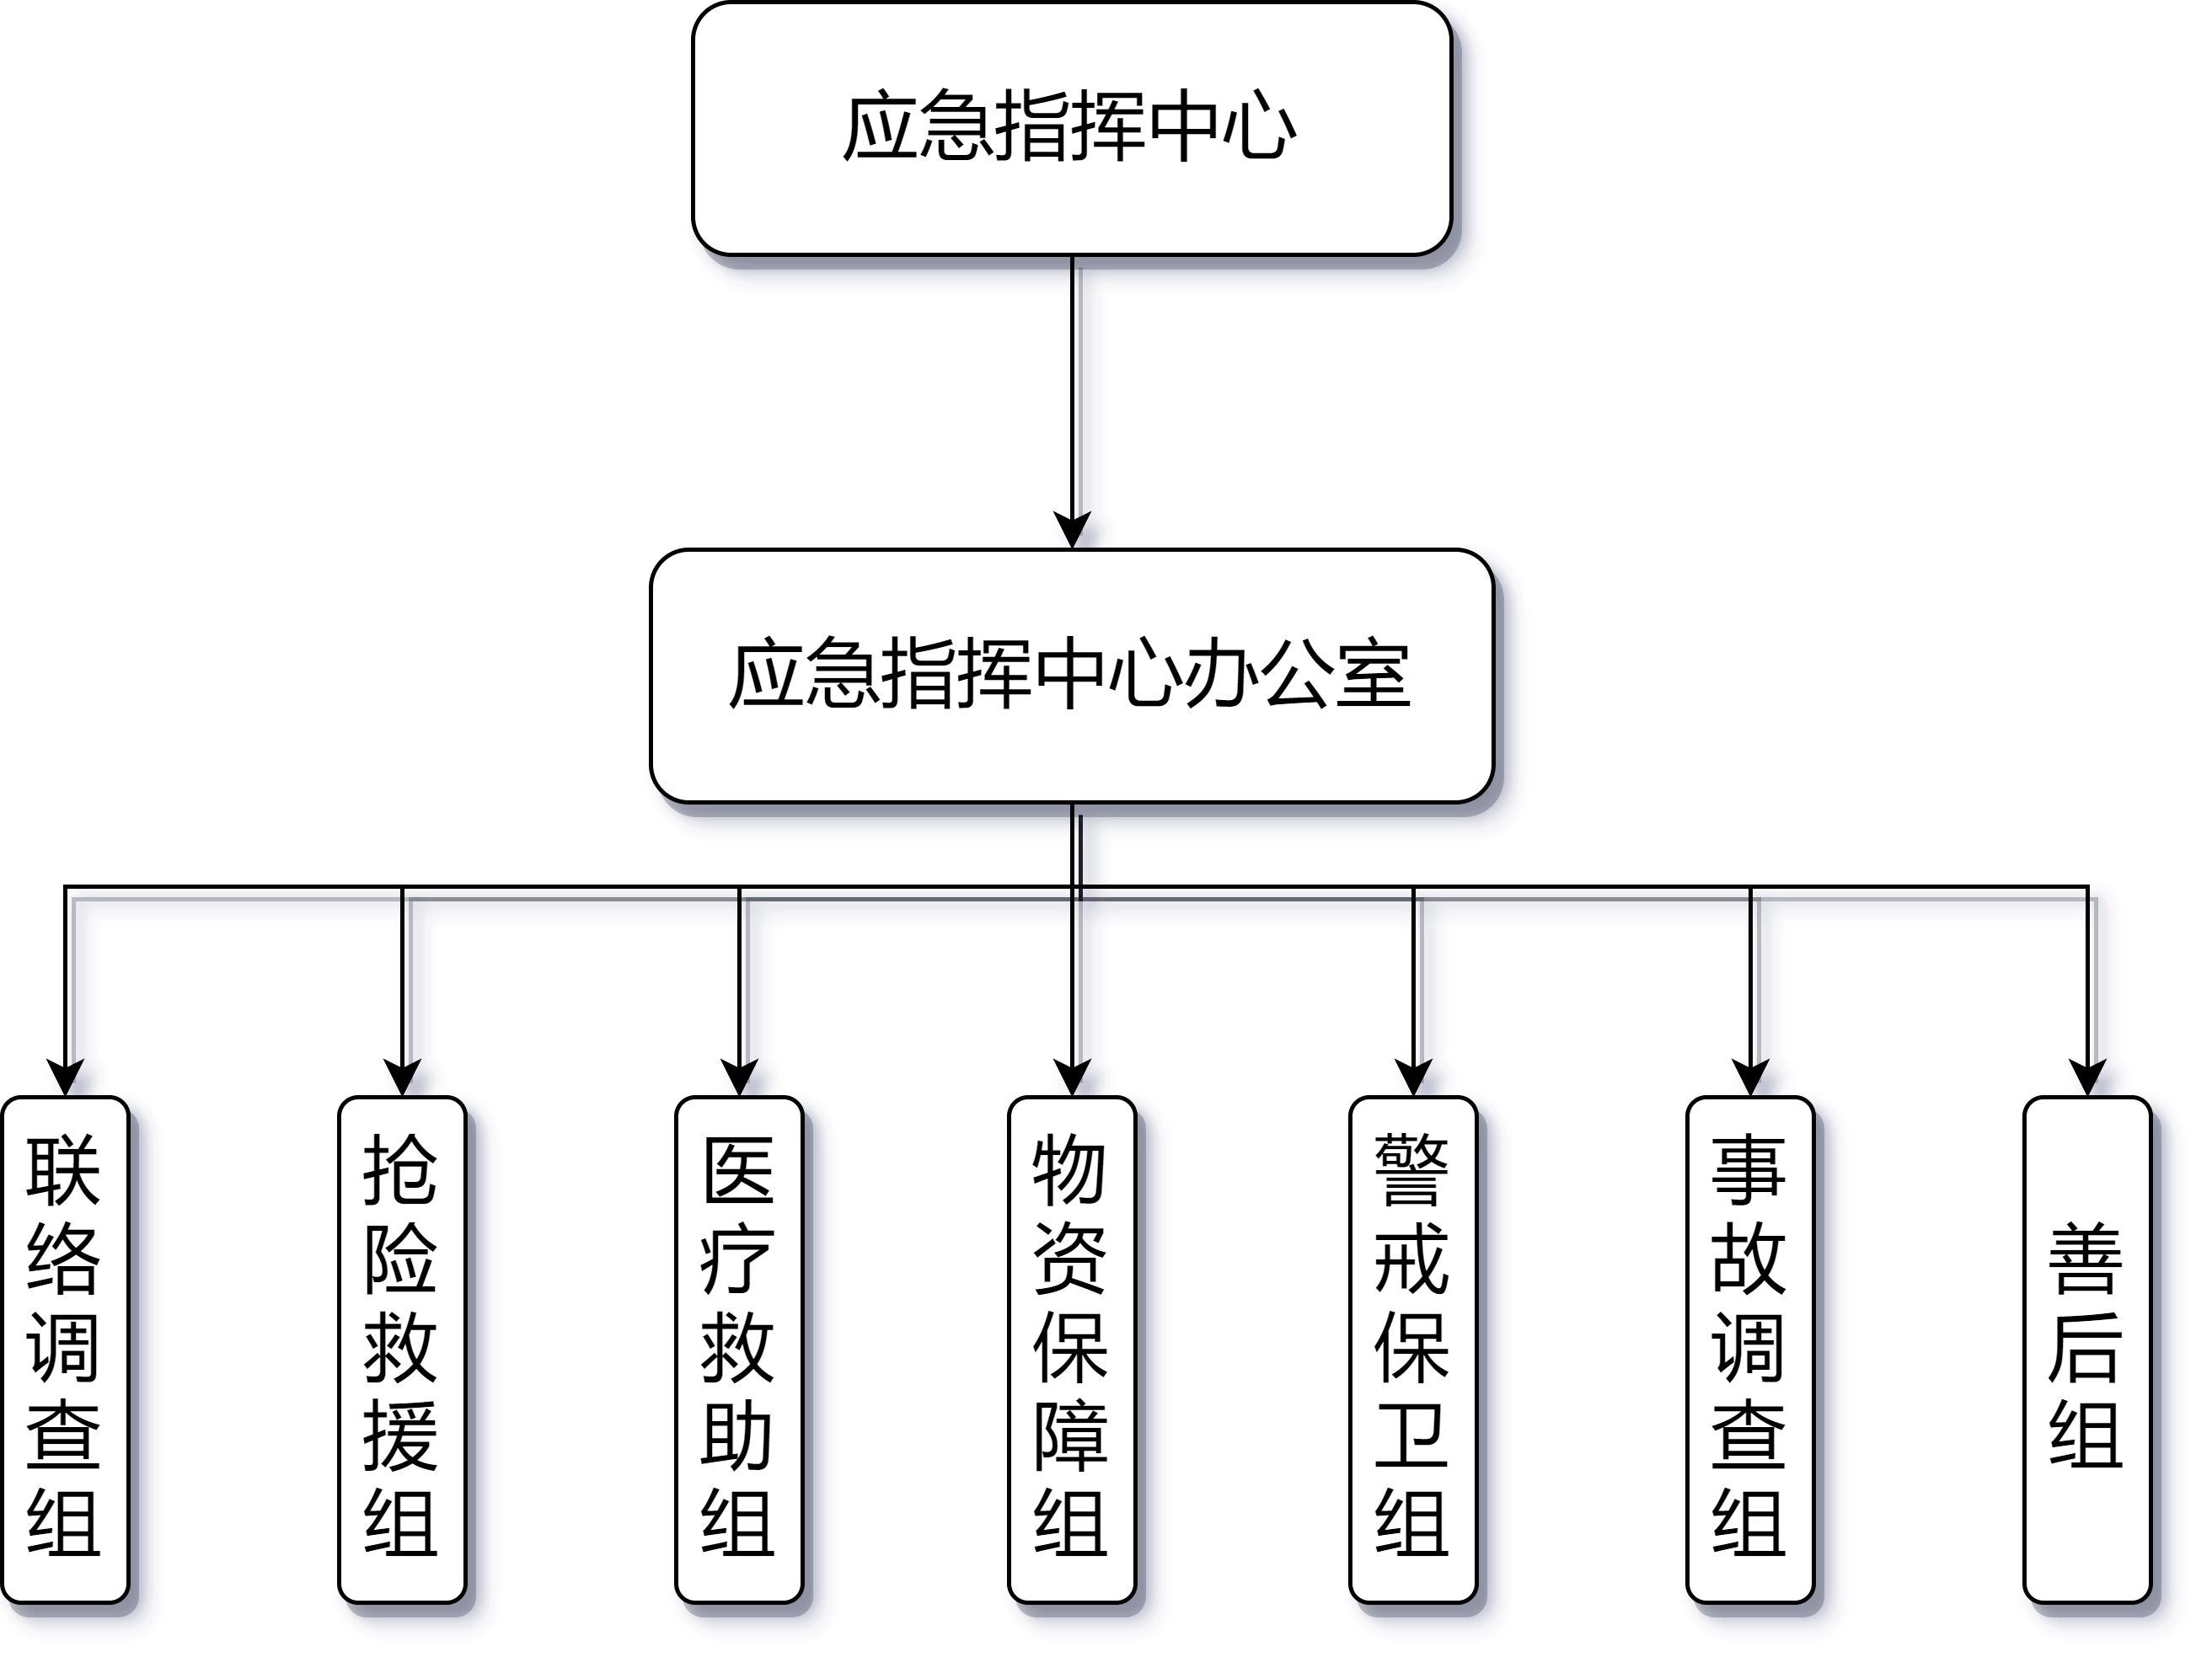
\includegraphics[width=0.8\linewidth]{figure/c8f1.png}
    \caption{项目应急指挥组织机构图}
    \label{fig:c8f1}
\end{figure}

各个组应互相紧密配合,统一领导,分工协作。处理事故时应坚持以为人本的原则,最大限度的保证人员的生命安全,控制事态发展,在确保尽可能最小化伤亡的前提下快速有效的展开救援。

\subsection{应急响应}
\subsubsection{响应分级}

根据事故严重程度、可能造成的后果以及可控性和恢复能力,项目部将应急响应级别原则上分为一级和二级两级。其中:

(1) 二级事故是发生事故险情,发生有可能影响工程正常施工或对施工有一定影响的事件时,可能导致人员受伤的或可能导致 1000 万元以下直接经济损失的事故,项目部能够自己处理的事故;

(2) 一级事故是指发生事故,发生直接导致施工中断或对施工造成极大影响的,导致有 3 人以上被困的或有人死亡或重伤的、导致 1000 万元以上直接经济损失的,项目部无法自行处理的,需要相关部门紧急救援的事故。 

\subsubsection{响应程序}

事故发生后,出事地点相关负责人立即向指挥中心报告险情,并同时启动现场处置方案,指挥中心接到报警后立刻对险情进行评估,确定响应等级并启动预案,详细的
响应流程见图 \ref{fig:c8f2}

\begin{figure}[thbp!]
    \centering
    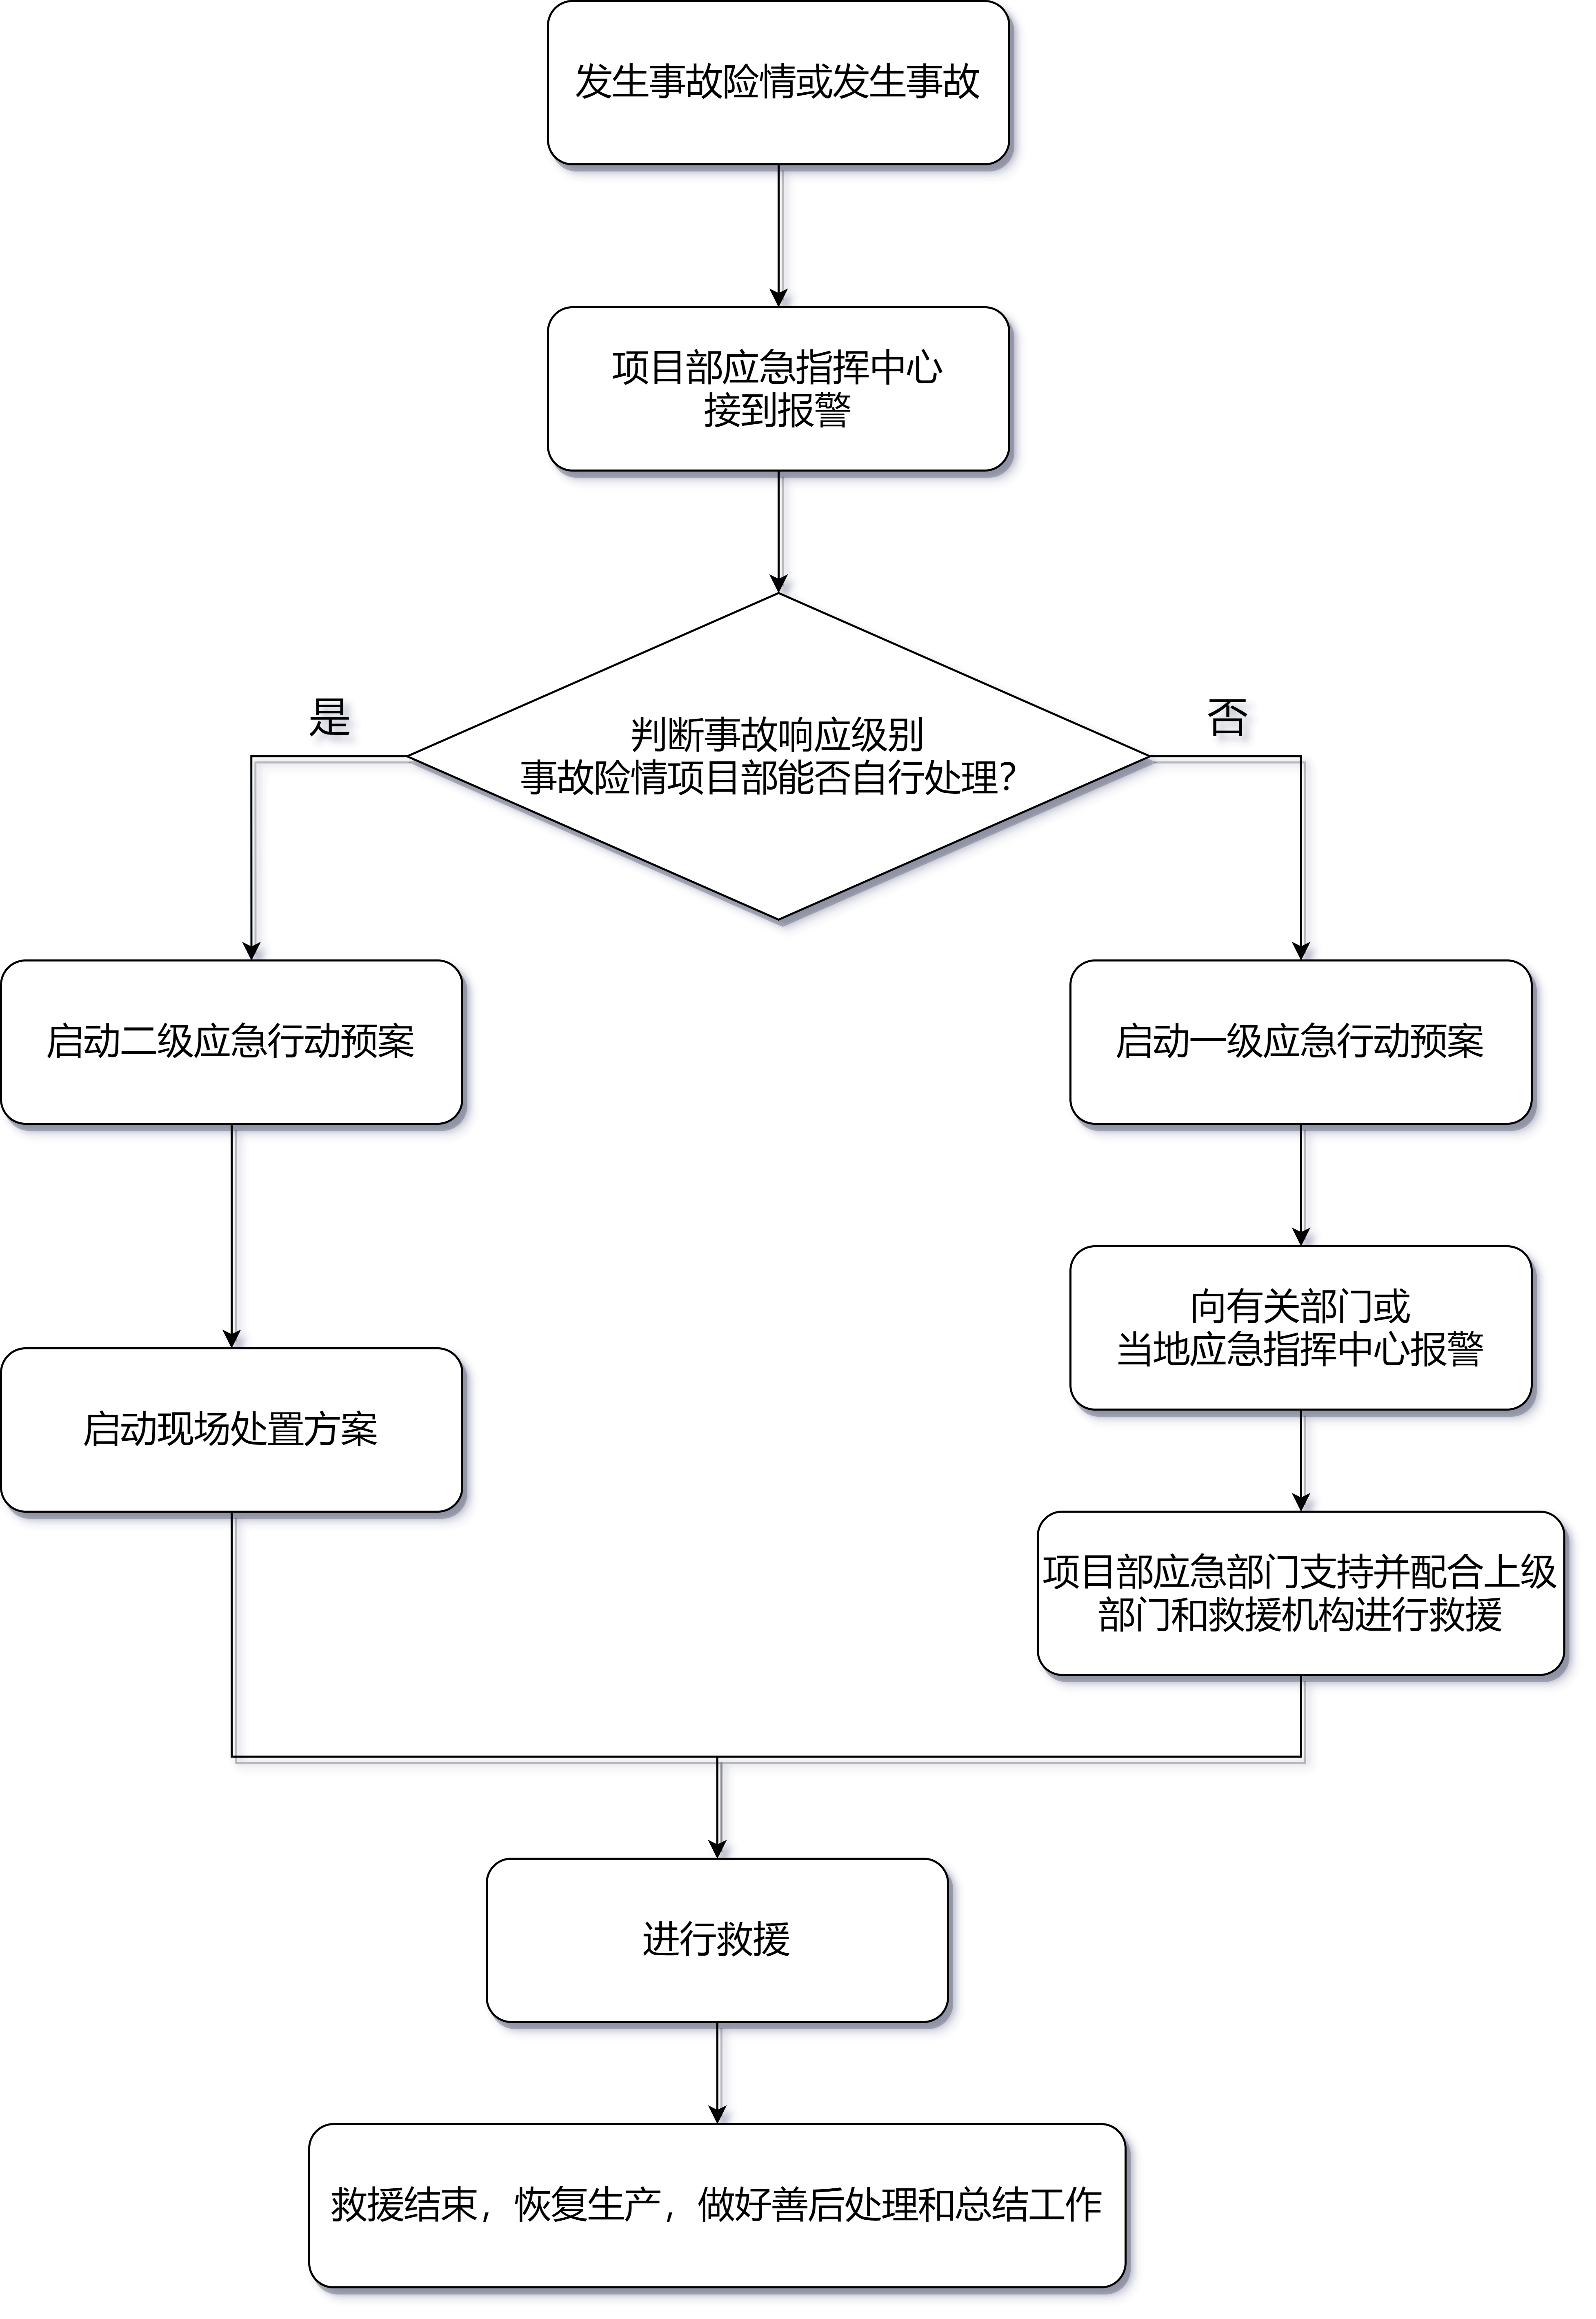
\includegraphics[width=0.8\linewidth]{figure/c8f2.png}
    \caption{项目应急响应程序流程图}
    \label{fig:c8f2}
\end{figure}

\subsection{事故应急处置}

\subsubsection{二级响应处置措施}

发生事故险情后,经指挥部确认该事故为二级事故,启动二级响应,抢险救援组率先将可能发生事故的部位接管并组织相关人员撤离,根据现场情况, 调整调集人员、设备与物质排查险情。
在响应处置过程中:

(1) 联络调度组负责维护现场秩序,将相关人员转移至安全地带,对有可能发生危险的区域进行有效的隔离;

(2) 医疗救助组负责现场的医疗抢救工作,随时待命,若发生事故则立即对受伤人员进行紧急处理,随后送往医院;

(3) 抢险救援组和物资设备保障组负责应急救援方案的主要实施,并由后勤保证组保证必要的通讯、抢救物质与设备以及自己及时到位

(4) 事故调查组在险情之后进场调查收集发生事故险情的相关资料,掌握施工险情情况,查明原因,评估事故的损失并
分清事故责任,提出防止事故发生的意见和建议,并做好书面报告。

(5) 全部疏散,安顿后停工观察,根据结果和进一步情况,明确安全等级并制定合理的复工复产计划。

\subsubsection{一级响应处置措施}

发生事故险情后,经指挥部确认该事故为一级事故,启动一级响应,抢险救援组率先将可能发生事故的部位接管并组织相关人员撤离,同时立即上报当地应急救援组织机构或地方人民政府相关机构,
应注意保护现场,已经撤离的人员不得再次靠近,等待有关部门组织专家和专业救援队伍前往现场并做好救援工作,同时,现场所有本项目部应急人员和应急小组应服从上级应急救援指挥机构的指挥。

\subsubsection{事故应急处置结束}

事故结束后,现场得以控制,次生与衍生灾害结束后,经过事故现场应急指挥机构批准后,现场应急状态结束。

应急状态结束后,又项目事故调查组负责收集事故资料,掌握事故状况,查明事故原因和评估事故影响程度和损失,查明事故责任并提出相应意见,以书面的形式汇报事故的详情,并提出防止事故再次发生的建议。

\subsection{事故后期处置}

事故处理结束后,现场应急指挥中心领导小组对现场要进行妥善的处理,包括证据的收集和现场的处理以及相关设施的重建并能尽快保证能够恢复生产,并要分析事故原因,总结经验教训,并采取预防措施。

\subsection{事故应急保障措施}
\subsubsection{应急队伍保障}

项目部应急管理中心下属的施工队每个队都应配备同等规模的应急小分队,平时项目部应加强对应急小分队的应急安全教育与培训,定期参观项目演练并亲自参与其中,做到一旦发生险情并能及时进入抢险救援状态,
能够顺利确保应急预案的有效实施。

\subsubsection{应急物资装备保障}

项目部应急指挥中心安排其下属的物资设备保障组负责项目的应急物资管理以及装备的储备及临时调配工作。

按照应急常态化的要求,物资设备保障组应当做到能够确定应急物资、设备和防护用品的数量,品类和状态,对有缺失,损坏和性能下降的物资以及耗材等应及时做好更新补充,维修和替换。

\subsubsection{其他保障}

(1) 交通运输

发生事故之后项目部应立即对现场和施工区域进行交通管制,为救援车辆和团队开辟应急特别通道,保障救援物资器材能及时准确的送达事故现场并能满足伤员的及时运出。

(2) 秩序与技术

应急响应时,又项目部警戒保卫组保障无关人员不得进入现场;同时要协助技术人员尽快倒搭现场,为救援队提供应激状态下的技术支持。

(3) 医疗与后勤

应急响应时,项目医疗救助组复制第一时间急救事故现场受伤人员,包括伤员的运出,现场对伤员的应急处置以及后续的输送伤员到正规医疗机构,直至伤员收到妥善救治;同时善后组负责后勤保障工作,协助整个
应急系统的正常运转,确保整个运转体系高效无虞。

\subsection{培训与演练}
\subsubsection{培训}

项目部应该对参加应急预案的各个部门和人员统一组织培训,目的在于发生险情时现在应急人员能够准确有效的进行应急处置,市应急救助人员具有充沛的应急救援知识和能力,培训磨合应急部门与其余部门的
协调和统一安排调度与指挥。

\subsubsection{演练}

在正式演练前,项目部应当召开演练前专项会议,协调各个部门的人员配备,并向参练人员明确其工作职责。项目部结合之前商定的元进行专项演练,对于在演练中发现的问题,应及时对预案的可行性进行整理和修改,
并杜绝相同问题在真正的应急救援中不再发生。

\subsection{火灾事故应急演练}
\subsubsection{指导思想}

通过举行火灾事故应急救援演练,事故风险较高部门和岗位的员工掌握突发火灾事故的应急救援程序、
消防器材操作使用方法和自救逃生方法,提高现场管理人员和救援人员的协调和快速应急反应能力,
从而进一步提高全体员工的自我保护意识和安全意识及自我保护能力。

\subsubsection{组织与安排}

(1) 演练领导小组\\

成员构成:配备配备总指挥一名和副总指挥一名

职责:负责演练活动筹备期间和实施过程中的领导与指挥工作。\\

(2) 演练策划组\\

成员构成:配备一名组长和三名组员

职责:负责制定演练方案以及对参与演练人员的指导和培训。\\

(3)	执行组\\

成员构成:配备一名组长和三名组员

职责:负责应急演练中与相关部门的联络、协调工作。负责情景事件要素设置及应急演练过程中的场景布置;负责调度参演人员、控制演练进程。\\

(4) 保障组\\

成员构成:配备一名组长和三名组员

职责:负责应急演练筹备及实施过程中安全保障方案的制定与执行;负责所需物资的准备,以及应急演练结束后上述物资的清理归库。\\

(5) 评估组\\

成员构成:配备一名组长和两名组员

职责:负责应急演练的评估工作,撰写应急演练评估报告,提出具有针对性的改进意见和建议。

\subsubsection{火灾应急演练过程}

安排 2 名工人在模拟火灾事故地点点燃烟雾弹,点燃烟雾弹后约 9 秒钟,一名员工随即大声呼救“着火了,请求马上救火”,现场另外一员工立即用对机向公司总指挥报告情况。

总指挥下令停止生产,全部人员立刻撤离现场,各生产部门员工在主管的带领下。从生产作业点快速撤离到预定的地点集结。随后各部门主管依次向总指挥报告人员疏散结果。
应急救援小组人员(灭火队员携带灭火器)从各方位赶到指挥中心前集合,各组长依次向总指挥报告。各救援小组人员在组长带领下奔向火灾现场展开应急救援。

6 名救护人员将 3 名伤者搀扶到保安室门口进行抢救,立即拨打 120 急救中心进行救援。

事故现场隔离现场保卫拉警戒带进行隔离,并指定进入的消防车从大门进入灭火地点,禁止其他无关车辆及人员进入。

各救援小组在组长带领下从事故现场向指挥台前集中并列队。组长向总指挥报告救援情况。

\subsubsection{演练要求}

(1) 公司全体员工应当认真学习有关消防安全知识,积极参与演练。

(2) 各救援小组由小组长组织相关人员学习救援器材的正确使用和相关救援措施,了解和掌握相关救援常识。

(3) 在演练过程中各救援小组要相互配合、协同作战,服从命令、听从指挥。

(4) )应急演练过程要力求紧凑、连贯,尽量反映真实事件下采取预警、应急处置与救援的过程。

(5) 应急演练应遵照应急预案有序进行。

\subsection{施工现场专项应急预案}
\subsubsection{高处坠落事故专项应急救援预案}

(1) 事故分析\\

高处坠落事故系以物体打击为主的多种因素导致的事故。\\

人员在施工过程有由于疏忽或失去平衡等因素发生高空坠落事故后会造成严重的人员伤亡或财产损失。\\

(2) 预防与监控\\

对作业人员要加强安全教育并做好交底工作。

高处作业时重点地区设立警示牌并避免上线同时作业

应加强对人员的安全教育,对高处作业、临边防护、吊装作业等重点项目进行安全检查,做到“早发现、早报告、早处置、低风险”\\

(3) 应急报告\\

当发生高处坠落事故时,应立即组织危险区域施工人员撤离,并报告应急指挥中心,同时指挥中心迅速评估险情,并决定是否应当启动应急预案,现场报警采取喊话的方式,向指挥中心
报告时应采用电话或对讲机。

项目应急安全中心应当使用电话向医院、公安、消防或当地的应急管理机构报告,报告的内容主要是:高处坠落事故发生的时间地点、背景、造成的经济损失、人员的伤亡状况以及需要额外救助的内容。\\

(4) 处置方式\\

当启动二级响应时,由项目部迅速启动救助方案;当启动一级响应时,应迅速撤离并报告有关部门并寻求帮助。\\

当发生高处坠落事故时,施工队应急自救小组启动机械伤害应急现场处置方案,抢险救援组迅速将遇险人员迅速撤离现场,且应当根据现场状况及时调整人员排布,设备用量,调集物资搜救被困人员

联络调度组负责维护现场秩序,将获救人员转移安全地带并有效隔离现场。

医疗救助组负责现场伤员的医疗工作,对救出的人员采取紧急医疗措施,受伤程度较轻的由医疗救助组先行急救,较重的迅速联系并送往医疗机构。

抢险救援组和物资保障组负责订正救援方案,并及时布置应急通讯、物资,并由后勤组保证所需物资和资金及时到位。

善后组负责妥善安置伤员,对在事故中罹难的职工按规定对其家属做好理赔工作。

事故调查组收集事故资料并掌握事故情况。评估事故影响程度和损失,查明主次要责任,提出复工方案与意见并形成书面报告。并由项目部应急负责人向上一级的应急救援组织机构汇报。\\

\subsubsection{机械伤害事故专项应急救援预案}

(1) 事故分析\\

机械伤害事故系以机械伤害为主的多种因素导致的事故。\\

机械在施工中,因检查维修不到位,操作违章,指挥有误等条件下,已发生碰撞,坠落等事故,造成人员伤亡和财产损失。\\

(2) 预防与监控\\

\quan{1} 项目部应制定安全管理制度,随时检查机械状态,对不符合要求的设备要及时调整,要对操作人员进行定期培训

\quan{2} 要根据现场的环境、气候或地形进行分析,对机械作业范围的高风险地区进行隔离并设立必要的警示牌

\quan{3} 机械运行中,如遇突发性的断电,偏离预定运行轨迹等故障时,应按照预设的方案及时应对,并通知施工队采取相应行动防止事故发生
有可能造成人员伤亡和财产损失时,应作出预警并向项目应急指挥中心回报并提出建议,项目预警指挥中心应做好启动应急预案的准备。\\

(3) 应急报告\\

当发生机械事故时,应立即组织危险区域施工人员撤离,并报告应急指挥中心,同时指挥中心迅速评估险情,并决定是否应当启动应急预案,现场报警采取喊话的方式,向指挥中心
报告时应采用电话或对讲机。

项目应急安全中心应当使用电话向医院、公安、消防或当地的应急管理机构报告,报告的内容主要是:机械伤害发生的时间地点、背景、造成的经济损失、人员的伤亡状况、机械的损坏程度以及需要额外救助的内容。\\

(4) 处置方式\\

当启动二级响应时,由项目部迅速启动救助方案;当启动一级响应时,应迅速撤离并报告有关部门并寻求帮助。\\

当发生一般机械伤害事故时,施工队应急自救小组启动机械伤害应急现场处置方案,抢险救援组迅速切断电源防止次生伤害并将遇险人员迅速撤离现场,且应当根据现场状况及时调整人员排布,设备用量,调集物资搜救被困人员

联络调度组负责维护现场秩序,将获救人员转移安全地带并有效隔离现场。

医疗救助组负责现场伤员的医疗工作,对救出的人员采取紧急医疗措施,受伤程度较轻的由医疗救助组先行急救,较重的迅速联系并送往医疗机构。

抢险救援组和物资保障组负责订正救援方案,并及时布置应急通讯、物资,并由后勤组保证所需物资和资金及时到位。

善后组负责妥善安置伤员,对在事故中罹难的职工按规定对其家属做好理赔工作。

事故调查组收集事故资料并掌握事故情况。评估事故影响程度和损失,查明主次要责任,提出复工方案与意见并形成书面报告。\\

当发生重大机械伤害事故时,现场负责人应立即切断所有电源设备,组织全部人员撤离危险地带,并由项目部应急负责人向上一级的应急救援组织机构汇报。

\subsubsection{火灾事故专项应急救援预案}

(1) 事故分析\\

火灾是由于动火不当而导致的事故。\\

在施工过程中火灾的隐患最大,特别是在施工的高峰期,明火作业交叉,易燃材料增多,用电负荷增大,极易引发火灾

生活区,库房等地发生火灾会造成严重的人员伤亡和经济损失,甚至造成大面积停工,设备损毁,甚至危害周边项目的正常生产生活。\\

(2) 预防与监控\\

\quan{1} 项目部应根据有关法律法规,制定完备的消防管理制度,并派专人检查制度的落实情况,消防器材的配备和维护情况,对不符合
消防安全要求的点要及时整改。

\quan{2} 要集合有关部门提供的火灾预警信息,结合当地有关自然状况,人口,交通,经济等因素进行分析评估,因地制宜的采取灾情预警和防范措施。

\quan{3} 当发现火灾苗头如烟、油、色以及气味异常时,应按照现场处置方案提前应对。并通知施工队采取相应行动防止事故发生
有可能造成人员伤亡和财产损失时,应作出预警并向项目应急指挥中心回报并提出建议,项目预警指挥中心应做好启动应急预案的准备。\\

(3) 应急报告\\

当发生火灾时,应立即组织危险区域施工人员撤离,并报告应急指挥中心,同时指挥中心迅速评估险情,并决定是否应当启动应急预案,现场报警采取喊话的方式,向指挥中心
报告时应采用电话或对讲机。

项目应急安全中心应当使用电话向医院、公安、消防或当地的应急管理机构报告,报告的内容主要是:火灾发生的时间地点、背景、造成的经济损失、人员的伤亡状况、燃烧物的种类或燃烧范围,以及需要额外救助的内容。\\

(4) 处置方式\\

当启动二级响应时,由项目部迅速启动救助方案;当启动一级响应时,应迅速撤离并报告有关部门并寻求帮助。\\

当发生轻微火灾时,施工队应急自救小组启动机械伤害应急现场处置方案,抢险救援组迅速切断电源防止次生伤害并组织项目消防队进行灭火,且应当根据现场状况及时调整人员排布,设备用量,调集物资搜救被困人员

联络调度组负责维护现场秩序,将获救人员转移安全地带并有效隔离现场。

医疗救助组负责现场伤员的医疗工作,对救出的人员采取紧急医疗措施,受伤程度较轻的由医疗救助组先行急救,较重的迅速联系并送往医疗机构。

抢险救援组和物资保障组负责订正救援方案,并及时布置应急通讯、物资,并由后勤组保证所需物资和资金及时到位。

善后组负责妥善安置伤员,对在事故中罹难的职工按规定对其家属做好理赔工作。

事故调查组收集事故资料并掌握事故情况。评估事故影响程度和损失,查明主次要责任,提出复工方案与意见并形成书面报告。\\

当发生严重火灾时,现场负责人应立即切断所有电源设备,组织全部人员撤离危险地带,并由项目部应急负责人立刻向当地消防部门和向上一级的应急救援组织机构汇报。

